\documentclass[11pt,a4paper]{article}
\usepackage[margin=1.65cm]{geometry}
\usepackage{amsmath,amssymb,booktabs,array,xcolor,tikz,enumitem,microtype,hyperref,fancyhdr,titlesec}
\usepackage[most]{tcolorbox}
\usetikzlibrary{arrows.meta,decorations.pathmorphing,decorations.pathreplacing,positioning,calc}
\definecolor{navy}{HTML}{183153}\definecolor{blue}{HTML}{2E6F9E}\definecolor{pale}{HTML}{EEF4F8}\definecolor{warn}{HTML}{FFF3D6}\definecolor{mist}{HTML}{FCE8E6}
\hypersetup{colorlinks=true,linkcolor=blue,urlcolor=blue}
\pagestyle{fancy}\setlength{\headheight}{14pt}\fancyhf{}\lhead{GCSE Physics · Sound \& Waves}\rhead{12 July 2026}\cfoot{\thepage}
\titleformat{\section}{\Large\bfseries\color{navy}}{}{0pt}{}[\color{blue}\titlerule]
\titleformat{\subsection}{\large\bfseries\color{blue}}{}{0pt}{}
\setlist{nosep,leftmargin=*}\setlength{\parindent}{0pt}\setlength{\parskip}{5pt}
\newtcolorbox{keybox}[1][]{breakable,colback=pale,colframe=blue,boxrule=.6pt,arc=1pt,title=\textbf{Key concept},#1}
\newtcolorbox{mistakebox}[1][]{breakable,colback=mist,colframe=navy,boxrule=.6pt,arc=1pt,title=\textbf{Common mistake},#1}
\newtcolorbox{examplebox}[1][]{breakable,colback=white,colframe=blue,boxrule=.8pt,arc=1pt,title=\textbf{Worked lesson example},#1}
\newcommand{\key}[1]{\begin{keybox}#1\end{keybox}}
\newcommand{\trap}[1]{\begin{mistakebox}#1\end{mistakebox}}
\begin{document}
\begin{center}
{\Huge\bfseries\color{navy} GCSE Physics — Sound \& Waves, Frequency, Amplitude}\par\vspace{5pt}
{\large Student: Phuc Nguyen \quad Tutor: Alex Kealy \quad Date: 2026-07-12}\par\vspace{4pt}
\textit{Source: Loom recording (full video analysis) + transcript · recording ID deafd2a7373946909782e184b2ac56e3}
\end{center}
\key{\textbf{Evidence boundary.} This guide follows the board-level whole-video analysis and the transcript. It preserves the questions, student response where recorded, Alex's correction, the taught method, and the final answer. The period example's decimal is explicitly marked as a completion because Alex wrote $1/0.6$ but did not finish it on screen. Brief real-world asides remain brief; no untaught physics has been added.}

\tableofcontents

\section{Sound begins with a vibration}
Alex began with sound because it gives a concrete way to see what all waves do. A loudspeaker does not throw pieces of air across the room. Its cone moves in and out. That motion produces alternating high- and low-pressure regions in the air, and the disturbance travels outwards until it reaches an ear or a microphone.

When Alex played the simulation at a low frequency, the cone could be seen moving in and out. Turning the amplitude down made the motion ``hardly moving''; increasing it made the cone travel much farther on each vibration. Increasing frequency made the heard note higher in \textbf{pitch}, while changing amplitude changed how loud the sound appeared in the demonstration. Phuc correctly separated the two ideas: frequency should not, by itself, be treated as volume.

The ear provides the final link in this chain. Pressure variations reach the eardrum, which responds to them. In Phuc's words, sound is ``a wave of pressure travelling in the air''; Alex confirmed that this was exactly the useful picture. A hand near a strong sound source can also feel those changing pressures.

\begin{keybox}[title=\textbf{The definition Alex built from the speaker}]
A \textbf{wave} is an oscillation or vibration that transfers \textbf{energy} from place to place without an overall transfer of \textbf{matter}. The air particles move backwards and forwards around their positions; they do not travel all the way from the speaker to the listener.
\end{keybox}

Phuc then asked why vibration counts as energy transfer. His reasoning was that a vibration can make another object vibrate, giving it kinetic energy. Alex agreed. The chain is therefore: vibrating source $\rightarrow$ neighbouring particles oscillate $\rightarrow$ the disturbance is passed on $\rightarrow$ a distant object can be made to vibrate.

Alex's crowd analogy makes the ``energy, not matter'' distinction memorable. In a Mexican wave, each person rises and sits in the same seat, yet the wave travels around the stadium. The people correspond to particles; the travelling pattern corresponds to the transferred energy. Likewise, dropping a stone in water produces wavefronts spreading out even though the water does not all move away with the front.

\trap{Do not say that air travels from the loudspeaker into the ear. Individual particles oscillate locally. It is the pressure disturbance and energy that travel. Also do not merge pitch and loudness: the lesson linked pitch to frequency and used amplitude to change loudness.}

\section{The particle picture: medium, compressions and rarefactions}
Sound requires particles to pass the disturbance from one place to the next. Alex called the substance carrying the wave a \textbf{medium}. Air is the lesson's main example. Without a medium there is no chain of neighbouring particles to pass on the sound vibration.

As the speaker cone moves out, it pushes nearby particles closer together. This makes a \textbf{compression}, a region in which particles are crowded. As the cone moves back, particles become more spread out, producing a \textbf{rarefaction}. Phuc used the idea that rarefaction is the opposite of compression to identify the two regions correctly.

\begin{center}
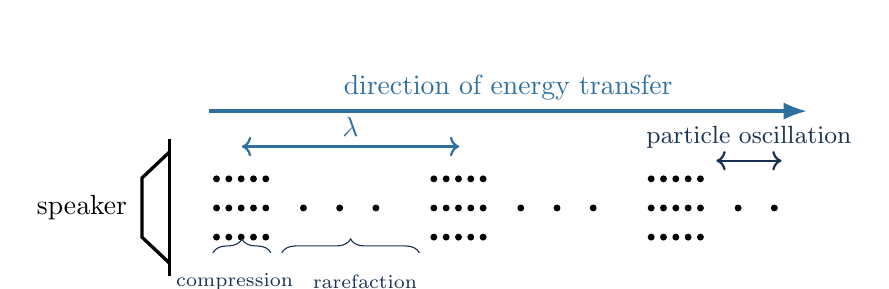
\begin{tikzpicture}[x=.92cm,y=1cm]
\draw[very thick] (0,.25)--(0,2.0);\draw[very thick] (0,.42)--(-.38,.75)--(-.38,1.5)--(0,1.83);
\node[anchor=east] at (-.45,1.12){speaker};
\foreach \x in {.65,.82,.99,1.16,1.33,3.65,3.82,3.99,4.16,4.33,6.65,6.82,6.99,7.16,7.33}{\foreach \y in {.75,1.12,1.49}{\fill (\x,\y) circle (1.25pt);}}
\foreach \x in {1.85,2.35,2.85,4.85,5.35,5.85,7.85,8.35}{\fill (\x,1.12) circle (1.25pt);}
\draw[-{Latex},blue,very thick] (.55,2.35)--(8.8,2.35) node[midway,above]{direction of energy transfer};
\draw[<->,navy,thick] (7.55,1.72)--(8.45,1.72);
\node[navy,font=\small] at (8.0,2.02){particle oscillation};
\draw[decorate,decoration={brace,amplitude=5pt},navy] (.6,.55)--(1.4,.55);
\node[navy,font=\scriptsize] at (.90,.18){compression};
\draw[decorate,decoration={brace,amplitude=5pt},navy] (1.55,.55)--(3.45,.55);
\node[navy,font=\scriptsize] at (2.70,.18){rarefaction};
\draw[<->,blue,thick] (1.0,1.9)--(4.0,1.9) node[midway,above]{$\lambda$};
\end{tikzpicture}
\end{center}

The repeating distance from the centre of one compression to the centre of the next compression is one wavelength. This matches the sine-like representation used on the board: successive compressions align with successive peaks, and rarefactions with troughs. The graph is a representation of the repeating disturbance; it does \emph{not} mean that air particles fly along a sine-shaped path.

\trap{A longitudinal-wave diagram is not showing a row of particles travelling to the right. The particles oscillate left and right; the pattern of compressions and rarefactions travels to the right. Do not call rarefaction ``refraction'': they are different words.}

\section{Reading a wave diagram: amplitude and wavelength}
The board displayed a particle model above a sine-like graph and asked Phuc to say everything he could about it. Alex then added four measurement arrows, deliberately including non-standard spans to test whether Phuc was using definitions rather than guessing.

\begin{center}
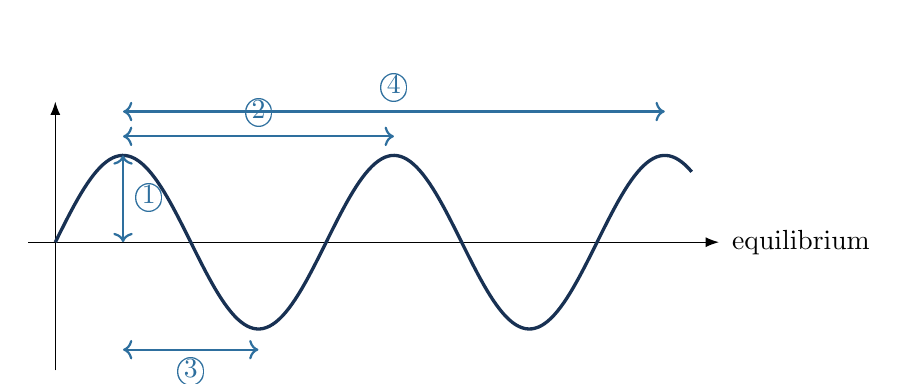
\begin{tikzpicture}[x=.86cm,y=1.05cm]
\draw[-{Latex}] (0,0)--(10.2,0);\draw[-{Latex}] (.4,-1.55)--(.4,1.7);
\draw[navy,very thick,domain=.4:9.8,samples=200] plot (\x,{1.05*sin(90*(\x-.4))});
\draw[<->,blue,thick] (1.4,0)--(1.4,1.05) node[midway,right]{\textcircled{1}};
\draw[<->,blue,thick] (1.4,1.28)--(5.4,1.28) node[midway,above]{\textcircled{2}};
\draw[<->,blue,thick] (1.4,-1.30)--(3.4,-1.30) node[midway,below]{\textcircled{3}};
\draw[<->,blue,thick] (1.4,1.58)--(9.4,1.58) node[midway,above]{\textcircled{4}};
\node[anchor=west] at (10.25,0){equilibrium};
\end{tikzpicture}
\end{center}

\begin{center}
\begin{tabular}{>{\bfseries}p{2.7cm}p{8.5cm}p{2.1cm}}
\toprule Quantity & Meaning used in the lesson & Unit \\ \midrule
Amplitude $A$ & Maximum displacement from the equilibrium (middle) position: middle-to-crest or middle-to-trough. & depends on graph \\
Wavelength $\lambda$ & Distance of one complete repeat between consecutive corresponding points, such as crest-to-crest or compression-to-compression. & m \\
Frequency $f$ & Number of complete waves passing a point each second. & Hz or $\mathrm{s^{-1}}$ \\
Period $T$ & Time taken for one complete wave to pass a point. & s \\ \bottomrule
\end{tabular}
\end{center}

Phuc correctly chose \textcircled{2} as wavelength, but was unsure whether \textcircled{4} might also be the requested distance. Alex confirmed that \textcircled{1} is amplitude and \textcircled{2} is wavelength. The deliberate catches were \textcircled{3} and \textcircled{4}: neither is a standard \emph{single} property as labelled. In cycle language, \textcircled{3} spans half a wavelength, while \textcircled{4} spans two wavelengths.

The word \textbf{maximum} matters in the definition of amplitude. A point halfway up the curve has a displacement, but not the amplitude. Likewise, wavelength is not ``a horizontal distance somewhere on a wave'': the endpoints must be at the same stage of the repeating pattern.

\trap{Do not measure amplitude from trough to crest; that is twice the amplitude. Do not measure wavelength from a crest to the next trough; that is only half a wavelength. Use corresponding points.}

\section{Transverse and longitudinal waves}
Alex classified waves by comparing two directions: the direction in which particles oscillate and the direction in which energy is transferred.

\textbf{Longitudinal waves} have oscillations \textbf{parallel} to energy transfer. Sound is the central example. A chosen air particle moves left and right along the same line in which the pressure disturbance travels, producing compressions and rarefactions.

\textbf{Transverse waves} have oscillations \textbf{perpendicular} to energy transfer. Alex used a rope: moving one end up and down makes the rope oscillate vertically while energy travels along it horizontally. He also used the stadium crowd, light/electromagnetic waves, and a simplified picture of ripples as lesson examples.

\begin{center}
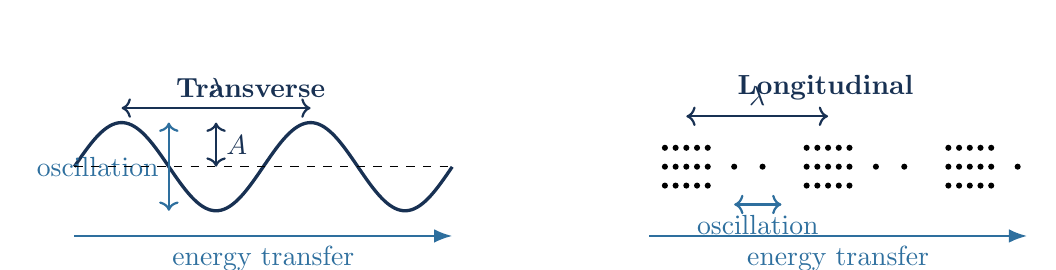
\begin{tikzpicture}[x=.8cm,y=.8cm]
\node[navy,font=\bfseries] at (2.8,2.5){Transverse};
\draw[navy,very thick,domain=0:6,samples=140] plot (\x,{1.25+0.7*sin(120*\x)});
\draw[-{Latex},blue,thick] (0,.15)--(6,.15) node[midway,below]{energy transfer};
\draw[<->,blue,thick] (1.5,.55)--(1.5,1.95) node[midway,left]{oscillation};
\draw[dashed] (0,1.25)--(6,1.25);
\draw[<->,navy,thick] (2.25,1.25)--(2.25,1.95) node[midway,right]{$A$};
\draw[<->,navy,thick] (.75,2.18)--(3.75,2.18) node[midway,above]{$\lambda$};
\begin{scope}[xshift=7.3cm]
\node[navy,font=\bfseries] at (2.8,2.5){Longitudinal};
\foreach \x in {.25,.42,.59,.76,.93,2.5,2.67,2.84,3.01,3.18,4.75,4.92,5.09,5.26,5.43}{\foreach \y in {.95,1.25,1.55}{\fill (\x,\y) circle (1.1pt);}}
\foreach \x in {1.35,1.8,3.6,4.05,5.85}{\fill (\x,1.25) circle (1.1pt);}
\draw[-{Latex},blue,thick] (0,.15)--(6,.15) node[midway,below]{energy transfer};
\draw[<->,blue,thick] (1.35,.65)--(2.1,.65) node[midway,below]{oscillation};
\draw[<->,navy,thick] (.59,2.05)--(2.84,2.05) node[midway,above]{$\lambda$};
\end{scope}
\end{tikzpicture}
\end{center}

In the rapid classification drill, Phuc correctly identified the Mexican wave as transverse and sound as longitudinal. He initially called light longitudinal; Alex corrected it to transverse. Phuc also initially classified a plucked guitar string as longitudinal because the sound it creates is longitudinal. Alex separated the two systems: the \emph{string itself} oscillates across the direction along the string, so its wave is transverse; the \emph{sound in air} is longitudinal. Ultrasound was then identified as longitudinal because it is sound.

Phuc asked about real water waves. Alex briefly noted that surface-water particle motion is actually a little circular, combining up/down and back/forth motion. He explicitly marked this as beyond what was needed and returned to the simplified transverse-versus-longitudinal classification model.

\trap{Always name what is waving. A guitar string carries a transverse wave, while the sound leaving it is longitudinal. Light is transverse. Do not define the types by the shape drawn on paper; compare oscillation direction with energy-transfer direction.}

\section{Frequency, period, pitch and amplitude}
Frequency answers ``how many complete cycles each second?'' Its unit, hertz, means per second: $1\,\mathrm{Hz}=1\,\mathrm{s^{-1}}$. Alex used a joke---if something happens too often, it ``hurts''---to attach the name hertz to frequency.

Period answers a different question: ``how long does one cycle take?'' If many cycles fit into each second, each cycle must take little time. If one cycle takes a long time, only a small number fit into each second. The quantities are reciprocals:
\[
\boxed{f=\frac{1}{T}}\qquad\text{and}\qquad\boxed{T=\frac{1}{f}}.
\]

\begin{examplebox}[title=\textbf{Lesson example: period to frequency}]
\textbf{Question:} A wave has period $T=0.6\,\mathrm{s}$. Determine its frequency.

\textbf{Alex's setup:}
\[
f=\frac{1}{T}=\frac{1}{0.6}.
\]
The board did not finish the decimal. Completing Alex's setup gives
\[
f=1.666\ldots\,\mathrm{Hz}\approx1.7\,\mathrm{Hz}.
\]
The $1.7\,\mathrm{Hz}$ is therefore a transparent arithmetic completion, not a claimed board answer.
\end{examplebox}

When Alex asked for the definition of frequency, Phuc first moved toward ``how long does it take to complete one cycle?'' Alex stopped him: that is period. Frequency is \emph{how many per second}. This correction also explains why frequency has unit $\mathrm{s^{-1}}$, whereas period has unit seconds.

For sound, the simulation linked higher frequency to higher pitch. Phuc wondered whether it also became louder, then correctly reasoned that frequency does not set the volume. Alex used amplitude to change the size of the cone vibration and the loudness. On a guitar, Alex connected pitch to changing the string's tension, thickness, or vibrating length; plucking the same string harder makes a bigger vibration and changes amplitude rather than its basic classification.

\trap{Do not swap period and frequency. ``Time for one'' means $T$ in seconds; ``number per second'' means $f$ in hertz. Do not say a high-frequency sound is automatically loud: the lesson treated frequency as pitch and amplitude as loudness/energy-transfer size.}

\section{Why wave speed equals frequency times wavelength}
Alex did not want the formula remembered as an isolated triangle. He started from the familiar relationship
\[
\text{speed}=\frac{\text{distance}}{\text{time}}.
\]
In one second, $f$ complete waves pass a point. Each complete wave has length $\lambda$. Therefore the distance represented in one second is $f\lambda$, giving
\[
\boxed{v=f\lambda}.
\]
The units make the same argument:
\[
\underbrace{\mathrm{m\,s^{-1}}}_{v}
=\underbrace{\mathrm{s^{-1}}}_{f}\times\underbrace{\mathrm{m}}_{\lambda}.
\]
Phuc successfully supplied that frequency means per second, wavelength is measured in metres, and metres times per second gives metres per second.

The three useful rearrangements are
\[
v=f\lambda,\qquad f=\frac{v}{\lambda},\qquad \lambda=\frac{v}{f}.
\]
Alex emphasised unit consistency: to obtain $v$ in $\mathrm{m\,s^{-1}}$, use $f$ in hertz and $\lambda$ in metres.

\begin{examplebox}[title=\textbf{Lesson calculation: microwave frequency}]
\textbf{Question 3(d):} A microwave has wavelength $0.15\,\mathrm{m}$ and travels through space at $300{,}000{,}000\,\mathrm{m\,s^{-1}}$. Find its frequency.

Phuc first mixed the two relationships, proposing that velocity was wavelength divided by frequency. Alex brought him back to ``speed is frequency times wavelength.'' The full route is:
\begin{align*}
v&=f\lambda &&\text{write the correct wave equation},\\
f&=\frac{v}{\lambda} &&\text{rearrange for the requested quantity},\\
f&=\frac{300{,}000{,}000}{0.15} &&\text{substitute with metres and seconds},\\
f&=2.0\times10^9\,\mathrm{Hz}. &&\text{state the answer and unit}
\end{align*}
A substitution check returns $(2.0\times10^9)(0.15)=3.0\times10^8\,\mathrm{m\,s^{-1}}$, the given speed.
\end{examplebox}

\key{Calculation routine modelled in the lesson: identify the requested quantity; write the formula; rearrange before inserting numbers; substitute; calculate; add the unit; then substitute back or inspect the scale.}

\trap{The period relationship $f=1/T$ and the wave-speed relationship $v=f\lambda$ are not interchangeable. In the microwave question, divide speed by wavelength. Keep $0.15$ in metres, and do not drop the hertz unit from the very large answer.}

\section{Sketching the same amplitude but double wavelength}
The graph task asked for a new wave with the \textbf{same amplitude} but \textbf{double the wavelength}. These instructions control different directions on the page.

\begin{enumerate}
\item ``Same amplitude'' fixes the vertical extent: the new crest and trough must reach the same heights as the original.
\item ``Double wavelength'' stretches the repeat horizontally: the new crest-to-crest distance is twice the old one.
\item Therefore, over a fixed graph width, the new wave completes half as many cycles. One new cycle occupies the space used by two old cycles.
\end{enumerate}

\begin{center}
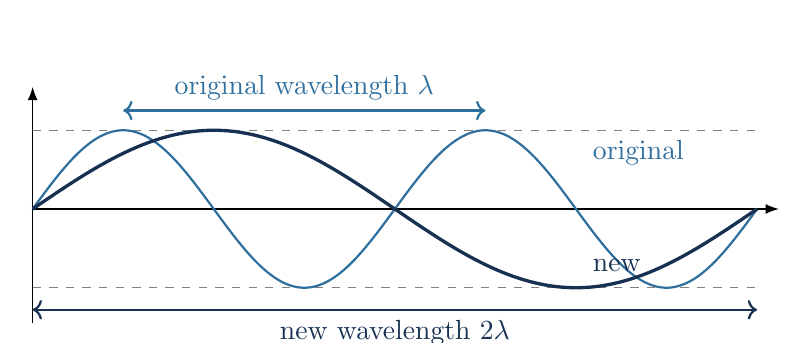
\begin{tikzpicture}[x=.92cm,y=1cm]
\draw[-{Latex}] (0,0)--(10.3,0);\draw[-{Latex}] (0,-1.45)--(0,1.55);
\draw[gray,dashed] (0,1)--(10,1);\draw[gray,dashed] (0,-1)--(10,-1);
\draw[blue,thick,domain=0:10,samples=240] plot (\x,{sin(72*\x)});
\draw[navy,very thick,domain=0:10,samples=240] plot (\x,{sin(36*\x)});
\draw[<->,blue,thick] (1.25,1.25)--(6.25,1.25) node[midway,above]{original wavelength $\lambda$};
\draw[<->,navy,thick] (0,-1.28)--(10,-1.28) node[midway,below]{new wavelength $2\lambda$};
\node[blue,anchor=west] at (7.6,.72){original};\node[navy,anchor=west] at (7.6,-.72){new};
\end{tikzpicture}
\end{center}

The diagram preserves exactly the board's qualitative instruction: same dashed amplitude limits, but a horizontally stretched navy curve. The axes had no numerical scale, so the task was about relationships, not reading values.

\trap{Do not double the wave's height: that would double amplitude, contrary to the question. Do not merely shift the curve sideways. Count complete cycles across the same width; the doubled-wavelength curve must show half as many.}

\section{Measuring the speed of sound}
Every method uses $v=d/t$, but the distance and timing procedure differ. Alex compared three board methods and asked for advantages or disadvantages rather than accepting a bare choice.

\subsection{Two microphones and a data logger}
Place microphones A and B a measured distance $d$ apart. Make a sound to the left of A. The computer records the instant the signal reaches each microphone and finds the arrival-time difference $\Delta t$. Then
\[
v=\frac{d}{\Delta t}.
\]
Phuc explained this correctly: record the time at A, record the time at B, subtract to obtain the time difference, and measure the separation.

Alex improvised values on the board. He first said $3\,\mathrm{cm}$, then corrected the intended separation to $30\,\mathrm{cm}$; the software example showed $0.01\,\mathrm{s}$. Using the corrected distance,
\[
30\,\mathrm{cm}=0.30\,\mathrm{m},\qquad v=\frac{0.30}{0.01}=30\,\mathrm{m\,s^{-1}}.
\]
Alex immediately noted that this is not close to the expected roughly $330\,\mathrm{m\,s^{-1}}$. The improvised values illustrated the calculation procedure, not a successful measurement.

\subsection{Long-distance visual signal}
A visible event and a sound are produced together at one end of a long distance. The observer starts timing when the event is seen and stops when the sound arrives. Alex described doing a version on a school sports pitch: people at one end clap above their heads so the timer can see the clap, then the sound reaches the other end.

For Alex's illustrative $100\,\mathrm{m}$ distance and expected $330\,\mathrm{m\,s^{-1}}$ speed,
\[
t=\frac{d}{v}=\frac{100}{330}\approx0.30\,\mathrm{s}.
\]
Phuc first stated $v=s/t$, then moved toward the needed rearrangement. Alex stressed that about three tenths of a second forces the human timer to react very quickly, although he recalled that the class activity was surprisingly accurate and enjoyable.

\subsection{Echo method}
Stand a known distance $d$ from a reflecting wall, make a sound, and time until the echo returns. The sound travels to the wall \emph{and back}, so its journey distance is $2d$:
\[
v=\frac{2d}{t}.
\]
The transcript preserves a board distance written/spoken as ``480'' in an echo example, but not enough associated unit/time detail to reconstruct a reliable final calculation. The secure lesson point is the factor of two for the return journey.

\begin{center}
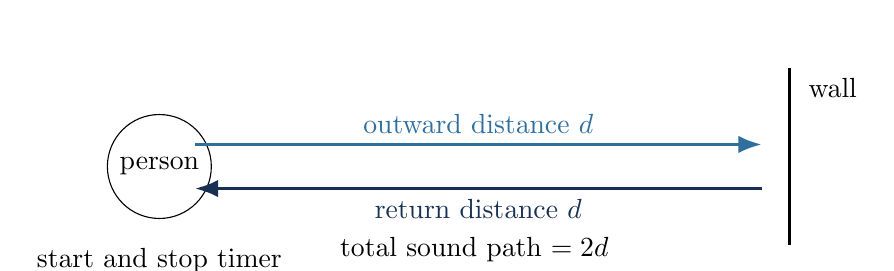
\begin{tikzpicture}[x=1cm,y=1cm]
\node[draw,circle,minimum size=.7cm] (P) at (0,0){person};
\draw[very thick] (8,-1)--(8,1.25);\node[anchor=west] at (8.12,1){wall};
\draw[-{Latex},blue,very thick] (.45,.28)--(7.65,.28) node[midway,above]{outward distance $d$};
\draw[-{Latex},navy,very thick] (7.65,-.28)--(.45,-.28) node[midway,below]{return distance $d$};
\node[below=7pt of P]{start and stop timer};
\node at (4,-1.05){total sound path $=2d$};
\end{tikzpicture}
\end{center}

When asked to choose, Phuc selected the data logger and said it was ``more accurate.'' Alex pressed: \emph{why} are the other two less accurate? He circled \textbf{REACTION TIMES}. Electronic detection removes the human delay in starting and stopping a stopwatch, whereas both manual methods depend on that delay.

\trap{Never write only ``the data logger is more accurate.'' Name the reduced uncertainty: human reaction time. In an echo calculation, do not use wall distance $d$ as the full journey; sound travels $2d$. Convert centimetres to metres before calculating a speed in $\mathrm{m\,s^{-1}}$.}

\section{Lesson retrieval drill and Phuc watch-list}
Alex's short retrieval checks exposed which distinctions need active recall.

\begin{center}
\begin{tabular}{p{4.1cm}p{4cm}p{6.1cm}}
\toprule Prompt & Phuc's attempt & Secure correction/outcome \\ \midrule
What creates sound? & ``Vibration'' & Correct: begin with a vibrating source. \\
What does sound need? & ``Something like air'' & Correct; general word: a medium/substance. \\
Compression or rarefaction? & Used opposites to choose & Correct: pushed together vs spread apart. \\
How many waves per second? & Asked for repeat, then frequency & Frequency, measured in Hz. \\
Mexican wave / sound & Transverse / longitudinal & Both correct. \\
Light & Longitudinal & Corrected: transverse. \\
Plucked guitar string & Longitudinal & String wave is transverse; emitted sound is longitudinal. \\
Microwave equation & $v=\lambda/f$ & Corrected to $v=f\lambda$, then $f=v/\lambda$. \\
Best speed method & Data logger: ``more accurate'' & Complete reason: removes human reaction-time uncertainty. \\ \bottomrule
\end{tabular}
\end{center}

A good redo routine is to cover the final column and answer each prompt aloud. For classification, always say both directions: ``oscillations are perpendicular/parallel to energy transfer.'' For calculations, write units beside each given value before selecting the equation. For practical explanations, finish the sentence ``because it reduces...'' with the named uncertainty.

\trap{Recognition is not the same as recall. Being able to agree with the correction is not enough: Phuc should reproduce the complete definition, equation, rearrangement and uncertainty explanation without seeing the final column.}

\section{What Alex asked to do next}
The lesson completed everything Alex had hoped to cover that day, but he said there was more to waves and that he would add more lessons for next time. Light would be discussed separately. Phuc also asked for a future lesson revising GCSE electricity because he felt less secure about circuits, potential energy and energy transfer; Alex agreed. No specific written waves homework or due date is evidenced in the supplied analysis/transcript.

\trap{Do not treat the end of this lesson as the end of the whole waves topic. Alex explicitly said there was more to cover. Electricity was a future-session request, not content taught in this guide.}

\clearpage
\section{One-page quick-recall summary}
\small
\begin{tabular}{>{\bfseries}p{3.0cm}p{8.1cm}p{3.5cm}}
\toprule Idea & Recall statement & Trigger/check \\ \midrule
Wave & Transfers energy without overall transfer of matter. & Mexican wave: people stay in seats. \\
Sound source & A vibration produces travelling pressure changes. & Speaker cone moves in/out. \\
Medium & Substance/particles that pass on the sound disturbance. & Air is the lesson example. \\
Compression & Region where particles are crowded together. & High-pressure region. \\
Rarefaction & Region where particles are spread apart. & Opposite of compression. \\
Amplitude $A$ & Maximum displacement from equilibrium. & Middle-to-crest, not trough-to-crest. \\
Wavelength $\lambda$ & One complete repeat between corresponding points. & Crest-to-crest or compression-to-compression; m. \\
Frequency $f$ & Number of waves per second. & Hz $=\mathrm{s^{-1}}$; higher sound frequency $\rightarrow$ higher pitch. \\
Period $T$ & Time for one complete wave. & Seconds; $f=1/T$. \\
Transverse & Oscillation perpendicular to energy transfer. & Light, rope, Mexican wave; guitar \emph{string}. \\
Longitudinal & Oscillation parallel to energy transfer. & Sound/ultrasound; compressions and rarefactions. \\
Wave equation & $v=f\lambda$. & Units: $\mathrm{m\,s^{-1}}=\mathrm{s^{-1}}\times\mathrm{m}$. \\
Period example & $T=0.6\,\mathrm{s}\Rightarrow f=1/0.6\approx1.7\,\mathrm{Hz}$. & Decimal completes Alex's setup. \\
Microwave example & $f=v/\lambda=(3.00\times10^8)/0.15=2.0\times10^9\,\mathrm{Hz}$. & Rearrange before substituting. \\
Graph change & Same amplitude, double wavelength. & Same height; half as many cycles across fixed width. \\
Two microphones & $v=d/\Delta t$. & Computer arrival-time difference; avoids stopwatch reaction time. \\
Visual method & Start on seeing signal; stop on hearing sound. & $100/330\approx0.30\,\mathrm{s}$: very short manual timing. \\
Echo & $v=2d/t$. & Out and back: double the wall distance. \\
Practical wording & Data logger is better because it removes human reaction-time error. & Never stop at ``more accurate.'' \\ \bottomrule
\end{tabular}

\vfill
\begin{keybox}[title=\textbf{If you remember only six things}]
(1) Waves transfer energy, not matter. \quad
(2) Sound is a longitudinal pressure wave requiring a medium. \quad
(3) $A$ is measured from equilibrium and $\lambda$ over one complete repeat. \quad
(4) Frequency is per second; period is time for one; $f=1/T$. \quad
(5) $v=f\lambda$. \quad
(6) In practical comparisons, name the reduced uncertainty: human reaction time.
\end{keybox}
\end{document}
